\chapter{Introduction}
\label{chap:intro}

\section{Cyber-physical systems}

The design of complex cyber-physical systems is an interdisciplinary process. From an engineering point of view, defining the requirements, designing sufficiently reliable components, dealing with scalability issues, employing testing processes that result in high test coverage, verifying safety critical components, and maintainability issues are all present at the same time. Systems engineering focuses on how to design and manage such systems. \cite{randomwikipedialink1}

Safety-critical systems are systems whose failure could result in loss of life, significant property damage, or damage to the environment. There are many well known examples for application in areas such as medicine, flight control, weapons industries, and nuclear systems. Many modem information systems are becoming safety-critical in a general sense because financial loss and even loss of life can result from their failure. Safety-critical systems will be even more common and more influential in the future. From a software perspective, the growing number of such systems result in the need for faster development cycles, which will require significant advances in areas like specification, architecture, and verification, to meet the safety requirements. \cite{safetycritical}

\section{Verification techniques}

As modern society is becoming more and more dependent on cyber-physical systems, the need for faultlessly working hardware and software increases. The development of safety critical systems require extensive testing efforts. Validation and verification methodologies have been present in the development processes of such systems for a long time \citep{ieee1012}, but faster and more reliable approaches are needed. Validation checks that the requirements specified for the software meet the needs of the user -- as such, validation usually can be aided, but can’t entirely be done by software. The point of verification is to analyse whether the specified requirements are met. Methods for verification can be divided into two groups: design time verification and runtime verification. These approaches aren't exclusive, and their mutual use can support a more robust verification process.

\subsection{Design time verification}

Design time verification is a method used for finding errors of the system before deployment. Traditional software development methodologies usually rely on design time approaches. Verification methods can be applied on multiple levels, from small parts to the whole entirety of the system. These processes check the compliance of the system against the specification of the appropriate level.\\
Formal verification can also be used to give proof that the verified parts match the behaviour described by the (also formal) specification. On the other hand, applying formal methods usually have higher costs, and the verification of complex systems can be impossible due to the problem of state space explosion. As a result, the role of formal methods is to verify the correct behavior of system components, and not the entire system.

\subsection{Runtime verification}

Runtime verification is a method for the inspection of running systems. The motivation of the approach is the complexity of design time verification. As systems are getting larger, the application of formal methods are more and more limited as the resources needed for verification cannot be realized. This means that formal verification methods must verify an abstract model, not the deployed system itself. In addition, specifications are rarely complete, and design time methods can rarely handle hardware errors.\\
Runtime verification uses monitors to observe certain (usually critical) components, checking whether their operation violates properties described by the specification. This has the advantage of detecting the erroneous operation of the system, and allowing systematic safety engineering for handling faults, or trigger an emergency shutdown if necessary.

\section{Systems engineering methods}

Traditional software development methods often use informal specifications to develop system, architecture, and component level designs which can also be informal. This can easily result in higher verification costs or faulty systems, making them suboptimal choices for safety critical software development. To introduce a level of formality and allow manageable, hierarchical software testing procedures, the V model was developed.

\subsection{V model}

A concept of operations is one of the initial stages in a system life cycle based on the “Vee” diagram, illustrated in \cref{fig:intro:vmodel}.

\begin{figure}[h]
	\centering
	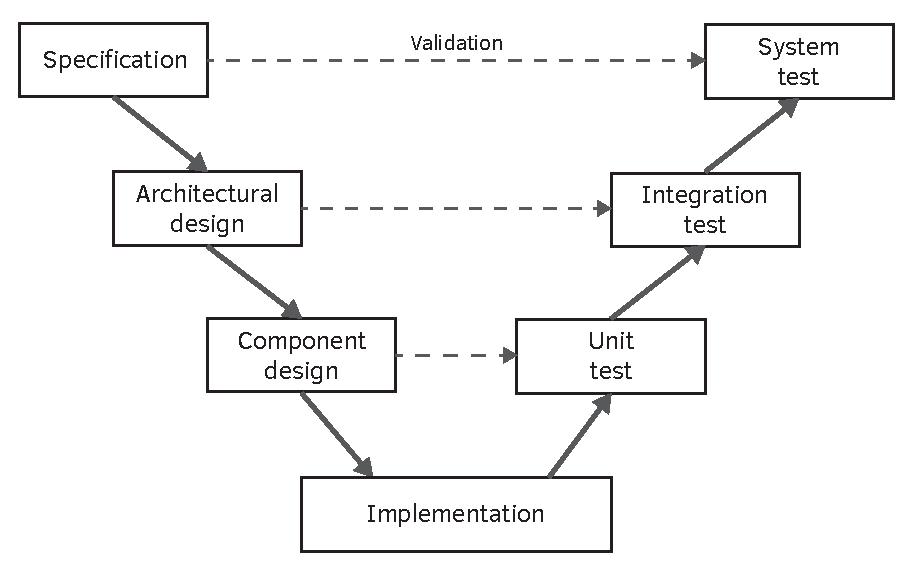
\includegraphics[width=0.8\linewidth]{include/figures/chapter_1/vmodel}
	\caption{The traditional V model \cite{vmodel}}
	\label{fig:intro:vmodel}
\end{figure}

\cref{fig:intro:vmodel} shows the stages of development, with a symbolic “V” showing the progression. The project definition stages on the left side begin with the development of a Concept of Operations, continue with Requirements and Architecture, and Detailed Design. The Implementation stage is shown across the base of the ``V'', with an arrow labeled ``Time'' pointing right to left across the bottom of the ``V''. The right side shows the testing and implementation stages of a system, with an upward-pointing arrow for progression. \cite{vmodel}

The V model is the basic scheme of a software development. In the left leg, we proceed down by decomposing the specifications into architecture level design, and the architecture design into component level designs. Every level of decomposition have it's own specifications. After the implementation process, we verify every levels of decompositions behavior with it's specification.


Model driven software development (MDSD) emphasizes problem solving by the development and maintenance of models describing the system being designed. MDSD heavily relies on automated code and documentation generation based on the models of components or the overall model of the system. 

Modeling has the advantage of introducing abstractions, thus reducing the complexity of the development process. Code generation guarantees that the code will inherit the properties that can be directly derived from the model, while reducing the costs by eliminating unnecessary round-trip engineering. The generation of documentation also results in the always up-to-date description of components, stored together with the requirements and the model. Furthermore, model based approaches have the advantage of easier testability, or if the model is formal enough they can make formal verification possible. This is especially important for the development of safety critical systems, making MDSD notably widespread in such areas.

Various methods and tools are available for the generation of test cases and monitoring components from models, as well as for formally verifying certain properties. These tools usually support the modeling formalisms used in their application domain.

MDSD is usually accompanied by the Y model -- a software life cycle model for component based systems \citep{ymodel}, extending the V model.

\subsection{Y model} % <3

\begin{figure}[h]
	\centering
	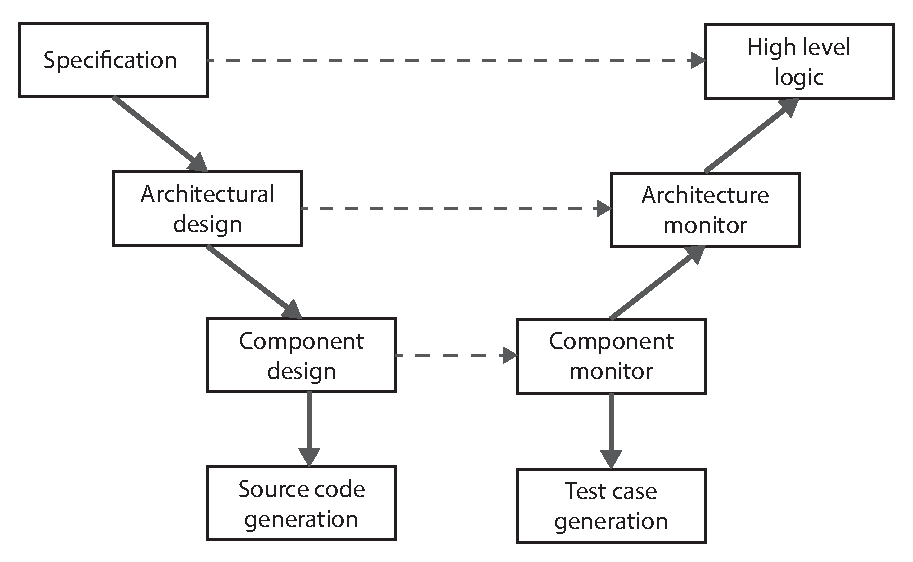
\includegraphics[width=0.8\linewidth]{include/figures/chapter_1/YModel}
	\caption{The Y model}
	\label{fig:intro:vmodel}
\end{figure}

The Y model \citep{ymodel} is an extension of the V model (which is in turn an extension of the waterfall model) \citep{randomwikipedialink3}, by using code and test case generation. Much like the V model, the development process is partitioned vertically. Each level contains a model that is transformed to a verification model, on which formal methods can be applied. The results of the verification process can be traced back to the original models making iterative improvement possible. The top level is for high level system models, while the second level contains architectural models, and the third one is for component based models. This provides input for the last step, source code and configuration generation for the individual components. Test cases are paired with the source code and can be generated from the component verification models.

\subsection{Modeling languages on different abstraction levels}

MDSD methods require modeling languages to describe the behavior of systems and components. Engineering practices developed a wide range of such languages over the years to support fast paced product development. This allows the use of domain specific languages, which leads to a shorter modeling process but challenges formal verification software, as their input is usually stricter and in a more general format. The result is the need for complex model transformations before the verification can begin, which can lead to higher development costs, or -- if the transformation contains errors -- even faulty behaviour.\\
As a result, standardized modeling languages were developed like the UML (Unified Modeling Language \citep{uml}) and SysML (Systems Modeling Language \citep{sysml}) languages.

\subsubsection{Finite automaton}

Formal modelling a system with finite state space is often done by using finite automata -- also known as finite state machines. A finite automaton accepts a (finite) list of symbols and produces a computation of the automaton for each input list.
Although finite automata can be easily visualized, this formalism describes a simple, flat transition system and lacks the support for higher level concepts. The development of finite automata models  are supported by many tools (e.g.: \citep{fsmd}).

\subsubsection{Statechart}

Statecharts, also known as state machines are an extension of finite automata. There are multiple available syntaxes for statecharts (e.g. the one defined by UML \citep{stcuml}). The higher level concepts that were introduced include variables, actions, and hierarchically nested states. Event-driven execution is also possible by using signals as the triggers of transitions. Available variable types heavily depend on the concrete semantics of the chosen statechart language. Actions can usually be variable assignments, signal raises, or the setting of timers. Hierarchy lets users organize system descriptions using a top-down approach. Support for hierarchy is introduced via nested states and parallel regions. States can also have entry and exit actions, which allows the description of common functionality in parent states \citep{stcmove}.\\
Statecharts are usually created by tools that support the graphical design of the model (e.g.: \citep{yakinduu}, an Eclipse based editor).


\subsubsection{Message Sequence Chart}

The formalism of message sequence charts (MSC) describes the communication between components -- the order in which messages can occur \citep{msc} \citep{msc2}. The message interchange is usually represented by a graphical model. These charts can be used for high level specification, design, trace based testing, or documentation. A collection of possible sequence charts can also describe a complete communication protocol between components. UML sequence diagrams were inspired by MSCs, but their semantics differ regarding some of the basic elements of the language such as lifelines and arrows \citep{mscuml}.

\subsubsection{Complex event processing}

\begin{figure}[h]
	\centering
	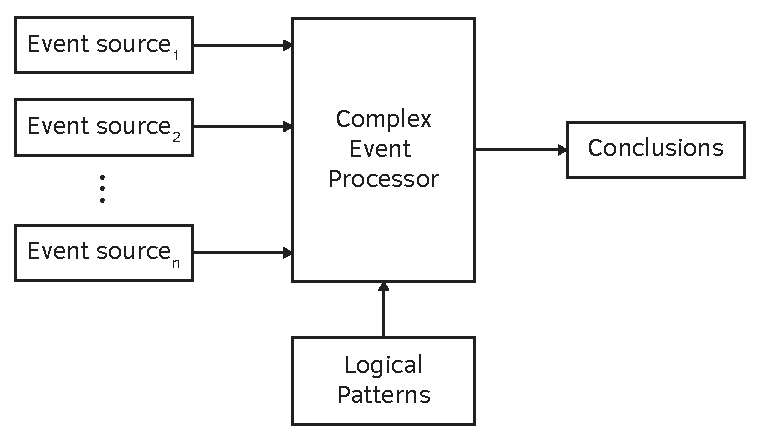
\includegraphics[width=0.7\linewidth]{include/figures/chapter_1/CEP}
	\caption{Complex event processing overview}
	\label{fig:intro:vmodel}
\end{figure}

Complex event processing is a method of tracking and analysing streams of information and deriving conclusions. In a complex event processing environment, there can be multiple event sources, and with logical patterns given by a formalism, we can find patterns in the incoming stream, e.g. events followed by another events in some sequence.

\section{A hierarchical approach to runtime verification}

We propose a hierarchical runtime verification approach by combining
\begin{enumerate}
\item traditional component-level monitors synthesized from statecharts with 
\item architecture-level monitors driven by complex event processing
\end{enumerate}

\begin{figure}[h]
	\centering
	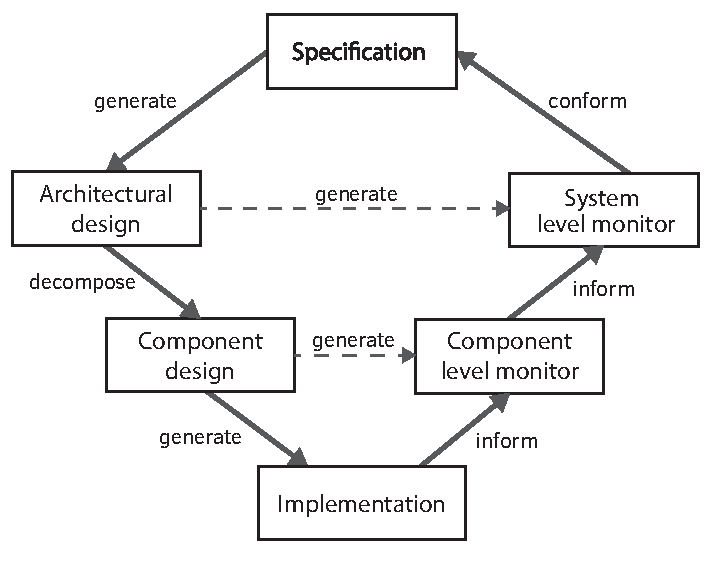
\includegraphics[width=0.8\linewidth]{include/figures/chapter_1/rv_vmodel}
	\caption{Hierarchical verification based on the V model}
	\label{fig:intro:rvmodel}
\end{figure}


Our goals were to provide:
\begin{itemize}
\item easy, high-level and precise specification languages for capturing monitors
\item automated synthesis of monitors
\item hierarchical monitoring
\end {itemize}

The result is a hierarchical runtime verification framework which can enable verification on two levels (\cref{fig:intro:concept_component}) The framework is capable of:
\begin{itemize}
  \item component level verification by monitors generated from a statechart formalism
  \item system level verification, that can be done by a complex event processing system
\end{itemize}
The monitors can generate messages indicating erroneous operation of the monitored components, while the complex event processing system can use the monitors' messages as atomic events for event patterns.

Additionally, the statechart language developed extends the usual statechart formalism by adding support for statechart templates. This enables users to easily describe systems with homogeneous components. The models can also be mapped to a formally verifiable transition system.

\begin{figure}[H]
	\centering
	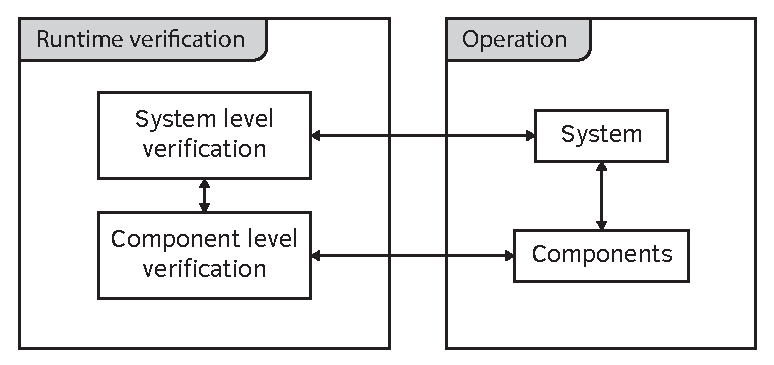
\includegraphics[width=0.65\linewidth]{include/figures/chapter_1/rv_overview}
	\caption{Associations between operation, and runtime verification components}
	\label{fig:intro:concept_component}
\end{figure}

With component level verification -- in out case with embedded monitors -- we can check the runtime state of each component. The system level verification observes the overall state of the system. If any of the components reports failure, we can make a decision based on the remaining components abilities to support the system verification. If we can provide safety despite component failures, the system can continue operation.

\begin{figure}[h]
	\centering
	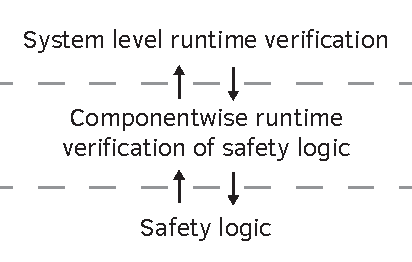
\includegraphics[width=0.4\linewidth]{include/figures/chapter_6/overview_1}
	\caption{Overview of the hierarchical runtime verification system}
	\label{fig:case_study:fov}
\end{figure}